\documentclass[xetex,mathserif,serif]{beamer}
\usepackage{polyglossia}
\setdefaultlanguage[babelshorthands=true]{russian}
\usepackage{minted}
\usepackage{tabu}
\usepackage{moresize}

\useoutertheme{infolines}

\usepackage{fontspec}
\setmainfont{FreeSans}
\newfontfamily{\russianfonttt}{FreeSans}

\definecolor{links}{HTML}{2A1B81}
\hypersetup{colorlinks,linkcolor=,urlcolor=links}

\setbeamertemplate{blocks}[rounded][shadow=false]

\setbeamercolor*{block title alerted}{fg=red!50!black,bg=red!20}
\setbeamercolor*{block body alerted}{fg=black,bg=red!10}

\tabulinesep=1.2mm

\title{Практика 11: веб-приложения}
\subtitle{Экспресс-курс}
\author[Юрий Литвинов]{Юрий Литвинов\\\small{\textcolor{gray}{yurii.litvinov@gmail.com}}}
\date{04.04.2022}

\newcommand{\attribution}[1] {
\vspace{-5mm}\begin{flushright}\begin{scriptsize}\textcolor{gray}{\textcopyright\, #1}\end{scriptsize}\end{flushright}
}

\begin{document}

    \frame{\titlepage}

    \section{Введение}

    \begin{frame}
        \frametitle{Веб-приложения}
        \framesubtitle{Как оно вообще работает}
        \begin{itemize}
            \item Пользователь заходит браузером на определённый URL
            \begin{itemize}
                \item На самом деле, выполняя HTTP GET-запрос на порт 80 или 443 (обычно)
            \end{itemize}
            \item ОС сервера перенаправляет запрос запущенному там \emph{веб-серверу}
            \begin{itemize}
                \item Например, Apache, IIS, нынче популярны также \emph{self-hosted} сервисы
            \end{itemize}
            \item Веб-сервер --- отдельный процесс, в рамках которого запущено несколько \emph{веб-приложений}, веб-сервер по URL запроса определяет, какому веб-приложению он адресован, и передаёт запрос ему
            \item Веб-приложение формирует ответ и отправляет его обратно по HTTP в виде HTML-страницы
            \item Эта страница и показывается пользователю в браузере
        \end{itemize}
    \end{frame}

    \begin{frame}
        \frametitle{Веб-сервисы}
        \begin{itemize}
            \item \textit{Веб-сервис} --- это примерно то же самое, но не для пользователя, а для других приложений
            \item Общаются не с помощью HTML, а посредством специализированных протоколов
            \begin{itemize}
                \item Например, SOAP
                \begin{itemize}
                    \item Использует синтаксис XML, может использовать HTTP как транспорт
                \end{itemize}
                \item Также популярны REST (это, правда, не протокол), gRPC
            \end{itemize}
            \item Содержат механизм публикации метаинформации
            \begin{itemize}
                \item Например, WSDL для SOAP
                \item OpenAPI (Swagger) для REST
            \end{itemize}
            \item Реализуются посредством технологий, например, ASP.NET Web APIs
        \end{itemize}
    \end{frame}

	\begin{frame}
        \frametitle{Типовой процесс разработки веб-приложения}
        \begin{itemize}
            \item Определяемся, можно ли сделать приложение client-only
            \item Определяемся с тем, какие запросы надо обрабатывать
            \item Пишем контроллеры и серверную логику
            \item Одновременно верстаем фронтенд, пишем клиентскую логику
            \item Настраиваем упаковку в Docker-контейнер, возможно, настраиваем оркестратор (например, Docker Compose)
            \item Проверяем всё локально
            \item Настраиваем облачное окружение, деплоим туда
            \item Настраиваем CI/CD
            \item Продолжаем процесс, пока не будем довольны результатом
        \end{itemize}
    \end{frame}

    \section{Фронтенд}

    \begin{frame}
        \frametitle{Браузерная часть}
        \begin{itemize}
            \item HTML (HyperText Markup Language) --- используется для задания содержимого и структуры веб-страницы
            \begin{itemize}
                \item Тут размечаются параграфы, заголовки, списки, таблицы и т.д.
                \item Тут же обычно определяются способы идентифицировать элементы
            \end{itemize}
            \item CSS (Cascading Style Sheet) --- используется для задания внешнего вида, оформления и расположения элементов
            \item JavaScript --- используется для задания поведения веб-страницы на клиенте
            \begin{itemize}
                \item Интерпретируется браузером
                \item К нему лучше относиться как к ``байткоду для браузера'', хотя можно писать на нём и руками
            \end{itemize}
        \end{itemize}
    \end{frame}

    \begin{frame}[fragile]
        \frametitle{DOM}
        \begin{itemize}
            \item DOM (Document Object Model) --- представление HTML-документа в виде дерева объектов и API для доступа к нему
            \item JavaScript может манипулировать DOM-деревом, браузер рендерит его ``на лету'', что и даёт интерактивность
        \end{itemize}
        \begin{columns}
            \begin{column}{0.5\textwidth}
                \begin{tiny}
                    \begin{minted}{html}
<table class="listing">
    <thead>
        <tr class="odd">
            <th>Выпускник</th>
            <th>Научный руководитель</th>
            <th>Текст</th>
        </tr>
    </thead>
    <tbody>
        <tr class="odd">
            <td>Акбаров Артур Александрович</td>
            <td>д.т.н., проф. Д.В. Кознов</td>
            <td><a href="bmo/441-Akbarov-report.pdf">Текст</a></td>
        </tr>
    </tbody>
</table>
                    \end{minted}
                \end{tiny}
            \end{column}
            \begin{column}{0.5\textwidth}
                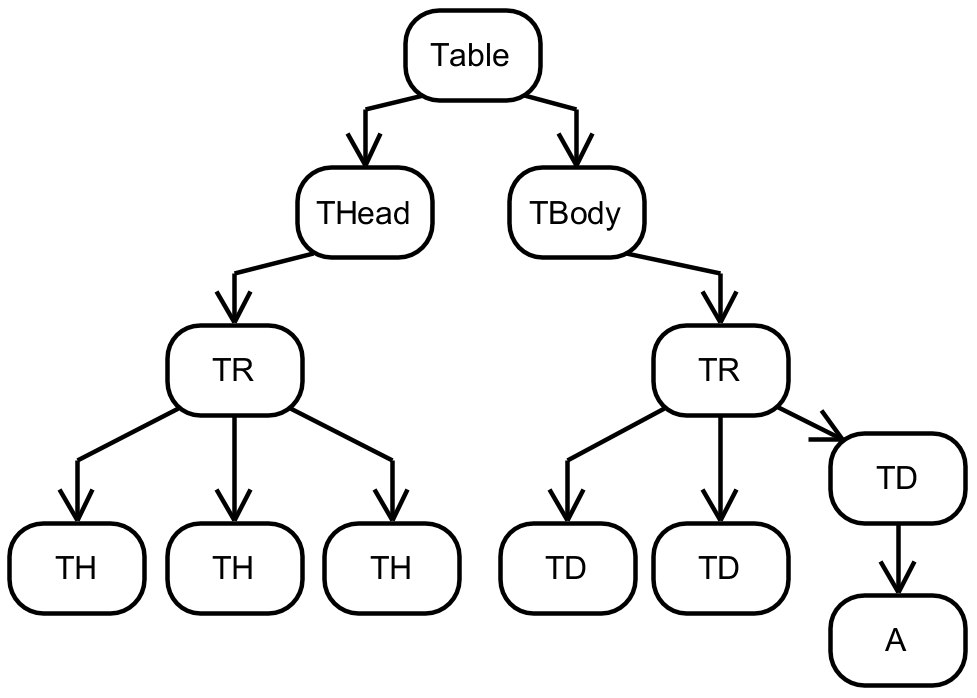
\includegraphics[width=\textwidth]{domTree.png}
            \end{column}
        \end{columns}
    \end{frame}

    \begin{frame}[fragile]
        \frametitle{HTML-формы}
        \begin{itemize}
            \item Способ получить ввод от пользователя
            \item Возможность организовать POST-запрос (GET по умолчанию)
        \end{itemize}
        \begin{minted}{html}
<form method="post">
  First name:<br>
  <input type="text" name="firstName"><br>
  Last name:<br>
  <input type="text" name="lastName"><br><br>
  <input type="radio" name="gender" value="male" checked>Male<br>
  <input type="radio" name="gender" value="female">Female<br>
  <input type="submit" value="Submit">
</form>
        \end{minted}
    \end{frame}

    \begin{frame}[fragile]
        \frametitle{CSS}
        \begin{itemize}
            \item Способ задать внешний вид элементов
        \end{itemize}
        \begin{minted}{html}
<!DOCTYPE html>
<html>
    <head>
        <style>
            body {background-color: powderblue;}
            h1   {color: blue;}
            p    {color: red;}
        </style>
    </head>
    <body>
        <h1>This is a heading</h1>
        <p>This is a paragraph.</p>
    </body>
</html>
        \end{minted}
        \attribution{https://www.w3schools.com}
    \end{frame}

    \begin{frame}[fragile]
        \frametitle{Или, что более типично}
        \begin{minted}{html}
<!DOCTYPE html>
<html>
<head>
  <link rel="stylesheet" href="styles.css">
</head>
<body>

<h1>This is a heading</h1>
<p>This is a paragraph.</p>

</body>
</html>
        \end{minted}
        \attribution{https://www.w3schools.com}
    \end{frame}

    \begin{frame}[fragile]
        \frametitle{Селекторы}
        \begin{minted}{html}
<p id="p01">I am different</p>
<p class="error">Error message</p>
        \end{minted}
        \vspace{5mm}
        \begin{minted}{css}
#p01 {
    color: blue;
}

p.error {
    color: red;
}
        \end{minted}
        \attribution{https://www.w3schools.com}
    \end{frame}

    \begin{frame}[fragile]
        \frametitle{Немного JavaScript-а}
        \begin{minted}{html}
<!DOCTYPE html>
<html>
<body>

<h1>My First JavaScript</h1>

<button type="button"
onclick="document.getElementById('demo').innerHTML = Date()">
Click me to display Date and Time.</button>

<p id="demo"></p>

</body>
</html> 
        \end{minted}
        \attribution{https://www.w3schools.com}
    \end{frame}

    \begin{frame}[fragile]
        \frametitle{Или так}
        \begin{small}
            \begin{minted}{html}
<!DOCTYPE html>
<html>
<head>
<script>
function doSomething() {
  document.getElementById("demo").style.fontSize = "25px";
  document.getElementById("demo").style.color = "red";
  document.getElementById("demo").style.backgroundColor = "yellow";
}
</script>
</head>
<body>

<button type="button" id="demo" onclick="doSomething()">Click me!</button>

</body>
</html>
            \end{minted}
        \end{small}
        \vspace{-3mm}
        \attribution{https://www.w3schools.com}
    \end{frame}

    \begin{frame}
        \frametitle{AJAX}
        \framesubtitle{Asynchronous JavaScript And XML}
        \begin{center}
            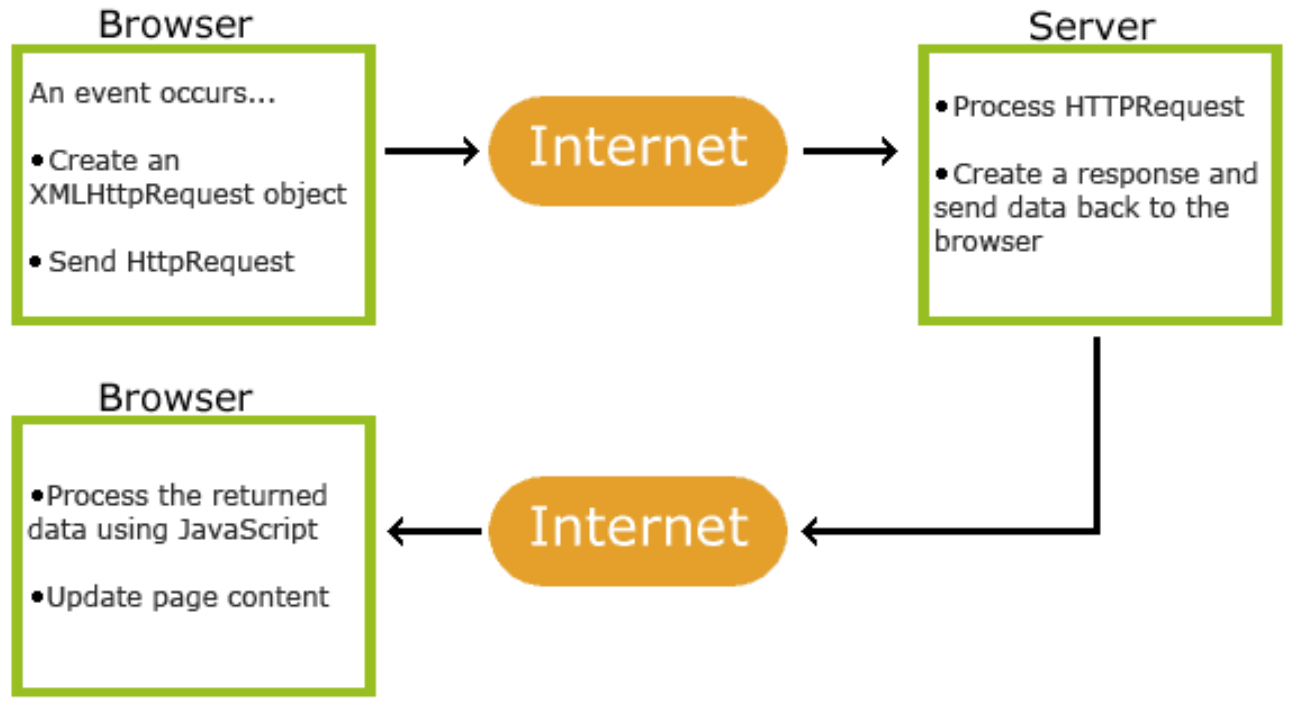
\includegraphics[width=0.7\textwidth]{ajax.png}
        \end{center}
        \attribution{https://www.w3schools.com}
    \end{frame}

    \begin{frame}[fragile]
        \frametitle{Пример}
        \begin{scriptsize}
            \begin{minted}{html}
<!DOCTYPE html>
<html>
<body>
<div id="demo">
  <h2>The XMLHttpRequest Object</h2>
  <button type="button" onclick="loadDoc()">Change Content</button>
</div>
<script>
function loadDoc() {
  var xhttp = new XMLHttpRequest();
  xhttp.onreadystatechange = function() {
    if (this.readyState == 4 && this.status == 200) {
      document.getElementById("demo").innerHTML = this.responseText;
    }
  };
  xhttp.open("GET", "ajax_info.txt", true);
  xhttp.send();
}
</script>
</body>
</html>
            \end{minted}
        \end{scriptsize}
        \vspace{-3mm}
        \attribution{https://www.w3schools.com}
    \end{frame}

    \begin{frame}[fragile]
        \frametitle{Fetch API}
        \begin{scriptsize}
            \begin{minted}{js}
const data = { username: 'example' };

fetch('https://example.com/profile', {
  method: 'POST', // or 'PUT'
  headers: {
    'Content-Type': 'application/json',
  },
  body: JSON.stringify(data),
})
.then(response => response.json())
.then(data => {
  console.log('Success:', data);
})
.catch((error) => {
  console.error('Error:', error);
});
            \end{minted}
        \end{scriptsize}
        \vspace{-3mm}
        \attribution{https://developer.mozilla.org/}
    \end{frame}

    \section{Бэкенд, ASP.NET}

    \begin{frame}
        \frametitle{.NET}
        \begin{itemize}
            \item По сути, альтернатива JVM от Microsoft
            \begin{itemize}
                \item Создавался с несколько другими целями
            \end{itemize}
            \item 2002 год, с тех пор раза три переписан
            \item Open source (MIT), кроссплатформенный, стандартизован
            \item Основные отличия от JVM:
            \begin{itemize}
                \item Понятие ``Сборка'', метаинформация
                \item Генерики --- полноценные типы
                \item Поддержка событий, асинхронности и т.п. в байт-коде
                \item Более спокойное отношение к обратной совместимости
            \end{itemize}
        \end{itemize}
    \end{frame}

    \begin{frame}
        \frametitle{C\#}
        \begin{itemize}
            \item Объектно-ориентированный язык общего назначения с сильной типизацией
            \begin{itemize}
                \item По сути, продвинутая Java
            \end{itemize}
            \item Основной язык программирования для платформы .NET
            \begin{itemize}
                \item Кроссплатформенный, open source, стандарт ECMA
            \end{itemize}
            \item Первая версия --- 2002 год, актуальная --- 08.11.2021, C\# 10
            \item 5-е место в индексе TIOBE на январь 2022
            \item Средства разработки
            \begin{itemize}
                \item Rider (\url{https://www.jetbrains.com/rider/})
                \item Microsoft Visual Studio (\url{https://www.visualstudio.com})
                \item Visual Studio Code (\url{https://code.visualstudio.com/})
                \item да любой удобный текстовый редактор
            \end{itemize}
            \item .NET SDK
        \end{itemize}
    \end{frame}

    \begin{frame}
        \frametitle{ASP.NET}
        \begin{itemize}
            \item Появился в 2002 году (вместе с самим .NET), переписан под .NET Core в 2016
            \item Кроссплатформенный, open-source, лицензия MIT
            \item Предполагает несколько моделей разработки:
            \begin{itemize}
                \item многостраничное приложение
                \begin{itemize}
                    \item с использованием паттерна MVC
                    \item с использованием Razor Pages (по сути, паттерна, Model-View)
                    \item на Server-side Blazor
                \end{itemize}
                \item одностраничное приложение (SPA)
                \begin{itemize}
                    \item на клиентских JS-библиотеках и Web APIs
                    \item на Client-side Blazor и Web APIs
                \end{itemize}
            \end{itemize}
            \item На самом деле, ``внутренности'' одинаковы, отличаются шаблоны и подходы
        \end{itemize}
    \end{frame}

    \begin{frame}
        \frametitle{ASP.NET MVC, основные понятия}
        \begin{center}
            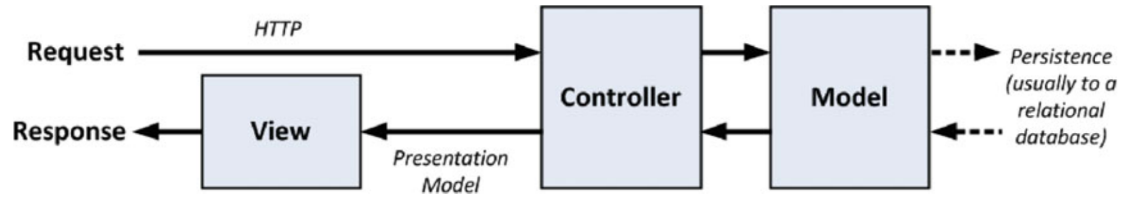
\includegraphics[width=0.7\textwidth]{mvc.png}
            \attribution{A. Freeman, Pro ASP.NET Core MVC}
        \end{center}

        \vspace{-5mm}

        \begin{itemize}
            \item \textbf{Модель} содержит или представляет данные, с которыми работает приложение
            \begin{itemize}
                \item \textbf{Domain model} содержит объекты предметной области вместе с бизнес-логикой, механизмами сериализации и т.д.
                \item \textbf{View Model} содержит классы, удобные для отображения во View, без бизнес-логики
            \end{itemize}
            \item \textbf{Представление} (View) отвечает за показ данных из модели пользователю
            \begin{itemize}
                \item Работает в браузере, но генерится на сервере
            \end{itemize}
            \item \textbf{Контроллер} отвечает за обработку входящих запросов, преобразование моделей и формирование данных для видов
        \end{itemize}
    \end{frame}

    \begin{frame}
        \frametitle{Конвейер обработки запроса}
        \begin{center}
            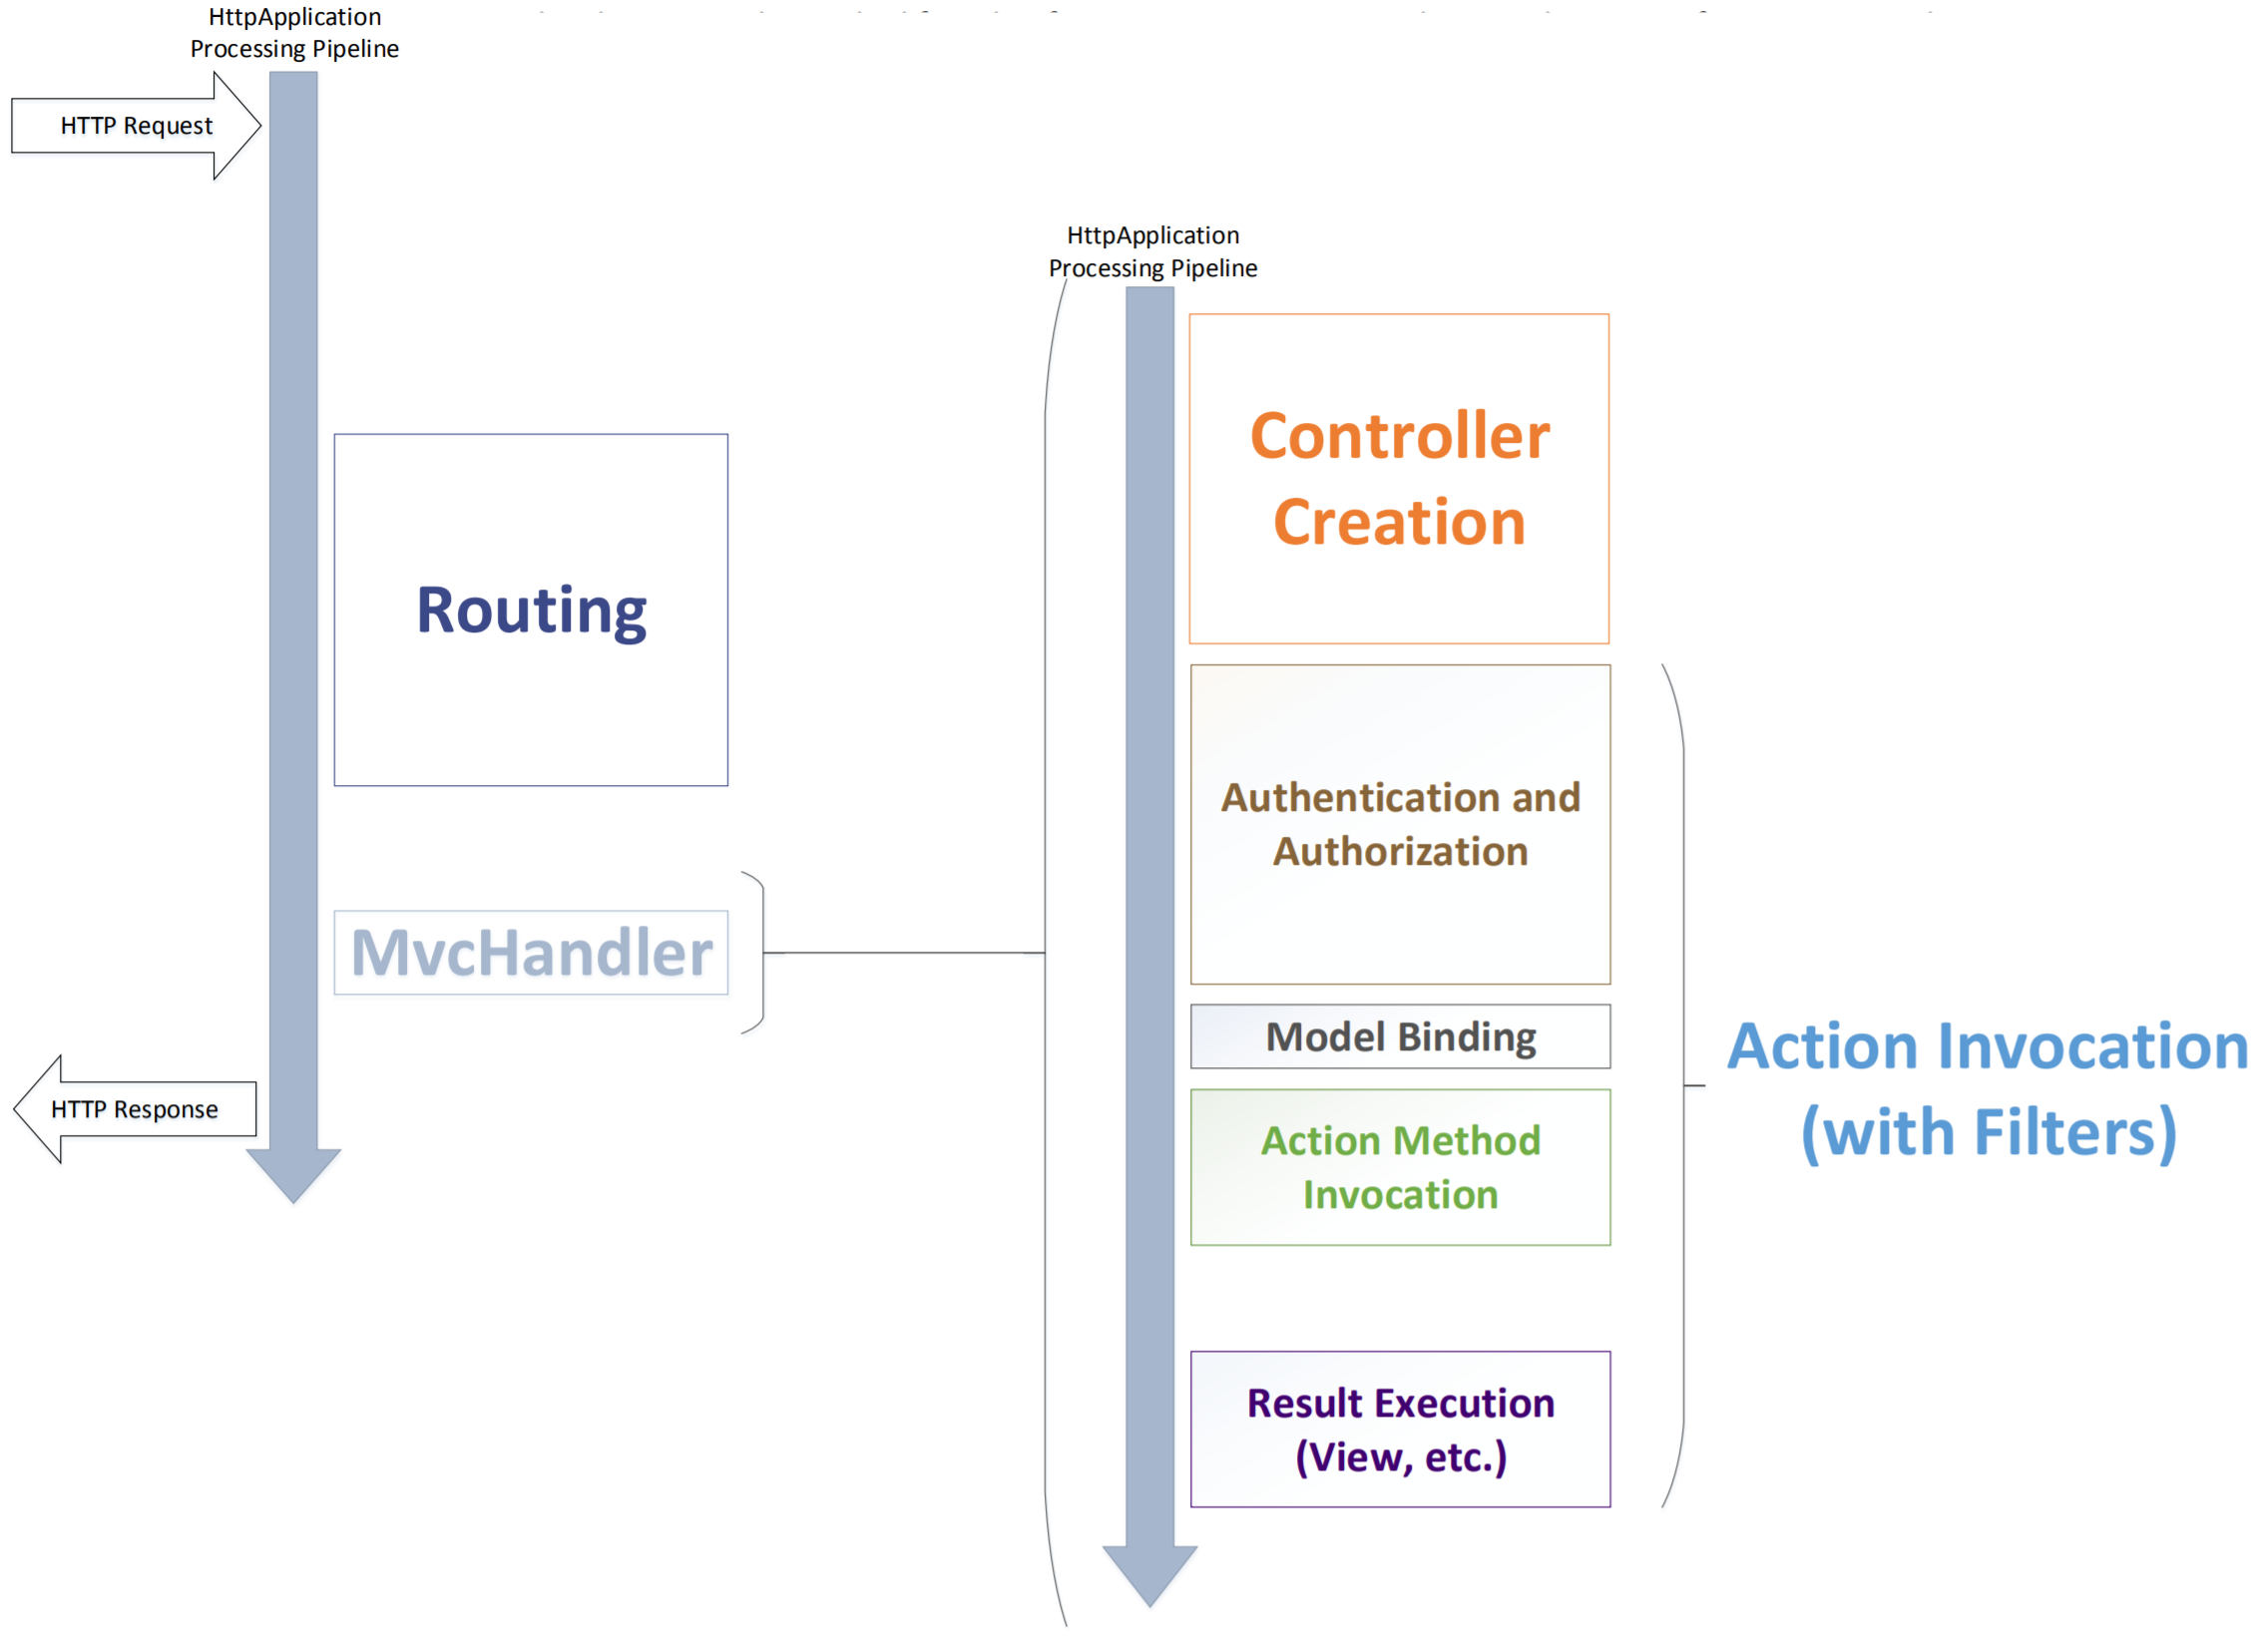
\includegraphics[width=0.85\textwidth]{requestLifecycle.png}
            \vspace{-5mm}
            \attribution{MSDN}
        \end{center}
    \end{frame}

    \begin{frame}
        \frametitle{Типичная структура проекта ASP.NET}
        \begin{itemize}
            \item На самом деле, два шаблона проекта:
            \begin{itemize}
                \item Web Application --- Razor Pages, ``облегчённая версия''
                \item Web Application (Model-View-Controller) --- ``классическая'' версия
            \end{itemize}
            \item \textbf{wwwroot} --- статические ресурсы приложения (то, что можно включать в html-страницу), отправляются клиенту как есть
            \begin{itemize}
                \item favicon.ico --- картинка, показывающаяся в заголовке вкладки
            \end{itemize}
            \item \textbf{Controllers} --- контроллеры, что неудивительно
            \begin{itemize}
                \item Принцип Convention-over-configuration
            \end{itemize}
            \item \textbf{Models} --- доменные и view-модели
            \item \textbf{Views} --- шаблоны HTML-страниц для представлений
            \begin{itemize}
                \item Подпапки должны соответствовать контроллерам
                \item Частичные представления
            \end{itemize}
            \item \textbf{appsettings.json} --- конфигурация приложения
            \item \textbf{Program.cs} --- конфигурирует хост, сервисы и запускает приложение
        \end{itemize}
    \end{frame}

    \section{Razor}

    \begin{frame}
        \frametitle{Razor}
        \begin{itemize}
            \item Язык задания правил генерации
            \begin{itemize}
                \item Обычно используется для генерации веб-страниц, но может использоваться и независимо
            \end{itemize}
            \item Состоит из текста на целевом языке (в нашем случае html), кода на C\# и Razor-разметки, которая собирает всё это воедино
            \item Сервер исполняет Razor-код, используя данные \textit{модели} для генерации итоговой html-ки, которую и отправляет клиенту
        \end{itemize}
    \end{frame}

    \begin{frame}
        \frametitle{Синтаксис Razor}
        \begin{itemize}
            \item HTML-разметка пишется как есть
            \item Блоки кода заключаются в \mintinline{text}|@{ }|
            \item Один оператор можно писать без скобок: \mintinline{text}|The time is @DateTime.Now|
            \begin{itemize}
                \item Обратите внимание, Razor-код выполняется на сервере!
            \end{itemize}
            \item Выражения можно заключать в круглые скобки: \mintinline{text}|@(someValue * 10)|
            \item Всё, что выводится через \mintinline{text}|@|, кодируется вызовом HttpServerUtility.HtmlEncode
        \end{itemize}
    \end{frame}

    \begin{frame}[fragile]
        \frametitle{Пример}
        \begin{minted}{csharp}
@page

<h1>Cthulhu fhtagn!</h1>

@for (int i = 0; i < 300; ++i)
{
    <p>Cthulhu fhtagn!</p>
}
        \end{minted}
    \end{frame}

    \begin{frame}
        \frametitle{Синтаксис Razor (2)}
        \begin{itemize}
            \item Razor сам пытается угадать, где разметка, а где код
            \begin{itemize}
                \item Но у него не всегда получается
            \end{itemize}
            \item После \mintinline{text}|@| и до пробела (или до конца оператора) --- код
            \item После открывающего тэга --- разметка
            \item После \mintinline{text}|@:| --- HTML-разметка
            \item \mintinline{text}|@* ... *@| --- комментарии (серверные, не отправляются клиенту)
            \item \mintinline{text}|@@| --- \mintinline{text}|@| в HTML (escaping)
        \end{itemize}
    \end{frame}

    \section{Модели}

    \begin{frame}[fragile]
        \frametitle{Модели}
        \begin{itemize}
            \item Всё, что выше, не сильно полезнее статической HTML
            \item Реальное веб-приложение использует данные из \emph{модели}
        \end{itemize}
        \begin{minted}{csharp}
@page
@using RazorPagesIntro.Pages
@model IndexModel2

<h2>Separate page model</h2>
<p>
    @Model.Message
</p>
        \end{minted}
    \end{frame}

    \begin{frame}[fragile]
        \frametitle{Code behind}
        \begin{small}
            \begin{minted}{csharp}
using Microsoft.AspNetCore.Mvc.RazorPages;
using System;

namespace RazorPagesIntro.Pages
{
    public class IndexModel2 : PageModel
    {
        public string Message { get; private set; } = "PageModel in C#";

        public void OnGet()
        {
            Message += $" Server time is { DateTime.Now }";
        }
    }
}
            \end{minted}
        \end{small}
        \attribution{MSDN}
    \end{frame}

    \section{Роутинг}

    \begin{frame}
        \frametitle{Роутинг}
        \framesubtitle{Или как ASP.NET находит по запросу страницу}
        \begin{itemize}
            \item Convention over configuration --- пока вы выполняете соглашения об именовании, по умолчанию всё происходит за вас
            \item Есть возможность конфигурировать роутинг вручную
            \item Соглашения Razor Pages:
            \begin{itemize}
                \item URL вида ``адрес сайта/'' или ``адрес сайта/Index'' отображаются в /Pages/Index.cshtml
                \item /Pages/Contact.cshtml --- URL вида ``адрес сайта/Contact''
                \item /Pages/Store/Contact.cshtml --- ``адрес сайта/Store/Contact''
                \item /Pages/Store/Index.cshtml --- ``адрес сайта/Store'' или ``адрес сайта/Store/Index''
            \end{itemize}
        \end{itemize}
    \end{frame}

    \begin{frame}[fragile]
        \frametitle{Глобальное переопределение роутов}
        Razor Pages:
        \begin{minted}{csharp}
var builder = WebApplication.CreateBuilder(args);

// Add services to the container.
builder.Services.AddRazorPages(
    options => options.Conventions.AddPageRoute("/Index", "/Ololo"));
        \end{minted}
        \vspace{5mm}
        MVC:
        \begin{minted}{csharp}
app.MapControllerRoute(
    name: "default",
    pattern: "{controller=Home}/{action=Index}/{id?}");
        \end{minted}
    \end{frame}

    \section{Model binding}

    \begin{frame}[fragile]
        \frametitle{Model binding}
        \framesubtitle{Или как передать в Code Behind параметры}
        \begin{small}
            \begin{minted}{html}
@page
@model WebApplication1.Pages.IndexModel
@addTagHelper *, Microsoft.AspNetCore.Mvc.TagHelpers

<html>
<body>
    <p>
        Enter your name:
    </p>
    <form method="post">
        Name: <input type="text" name="name" />
        <input type="submit" />
    </form>
</body>
</html>
            \end{minted}
        \end{small}
        (GET тоже будет работать)
    \end{frame}

    \begin{frame}[fragile]
        \frametitle{Способ 1: в параметрах обработчика}
        \begin{small}
            \begin{minted}{csharp}
namespace WebApplication1.Pages
{
    public class IndexModel : PageModel
    {
        public void OnGet()
        {

        }

        public void OnPost(string name)
        {
            Console.WriteLine(name);
        }
    }
}
            \end{minted}
        \end{small}
    \end{frame}

    \begin{frame}[fragile]
        \frametitle{Способ 2: через свойства}
        \begin{small}
            \begin{minted}{csharp}
[BindProperty]
public string Name { get; set; }

public void OnPost()
{
    Console.WriteLine(Name);
}
            \end{minted}
        \end{small}
    \end{frame}

\end{document}
